\newpage
\section{Comparison of three methods}
Next, we will analyze the time complexity and the final performance of the three methods given in the above paper.

\subsection{Performance in different graphs}

\begin{table}[h]
\centering
\begin{tabular}{ p{0.15\textwidth} | p{0.15\textwidth} | p{0.15\textwidth}| p{0.15\textwidth}| p{0.15\textwidth}}
     \hline
     Graph number & Initial intersections &  FD result & LS by nodes result & LS by edges result\\
     \hline
     \codeword{1} & 1 & 1 & 1 & 1 \\
     \hline
     \codeword{2} & 1 & 0.22 & 0.91 & 0.19 \\
     \hline
     \codeword{3} & 157 & 0.34 & 0.19 & 0.06 \\
     \hline
     \codeword{4} & 390 & 0.17 & 0.33 & 0.36 \\
     \hline
     \codeword{5} & 180 & 0.06 & 0.08 & 0.09\\
     \hline
     \codeword{6} & 447 & 1 & 1 & 1 \\
     \hline
     \codeword{7} & 3368 & 0.84 & 0.59 & 0.63\\
     \hline
     \codeword{8} & 7108 & 0.60 & 0.88 & 0.80 \\
     \hline
     \codeword{9} & 1173 & 1 & 0.83 & 0.21 \\
     \hline
     \codeword{10} & 20302 & 0.97 & 0.99 & 0.57\\
     \hline
     \codeword{11} & 102695 & 1 & 0.99 & 1 \\
     \hline
     \codeword{12} & 954832 & 1 & 1 & 0.73 \\
     \hline

\end{tabular}
\end{table}
Several remarks:

\begin{itemize}
    \item In the column of every method, we give the proportion between the final intersection numbers and the initial intersection numbers.
    \item We display the generating results in the form of a table. Note that if the image is invalid at the beginning, we will call the previous generating method, which will cause the initial number of intersections of each image to be different, but after testing, such small differences in the image have little effect on the final algorithm result. So, for each graph, we will randomly use the number of intersections after the legalization process. 
    \item In the algorithm, if the final number of intersections is greater than the initial number of intersections, the initial image is returned. So the result 1 indicates that the number of intersections is unchanged or rising.
\end{itemize}
Observing the table, we find:
\begin{enumerate}
    \item The optimal result of more than half of the images is obtained by the LS by edges algorithm, which can show that this algorithm is generally effective;
    \item However, for Graph 5, the FD method is very useful which depends on its structure. We can see more intuitively these four methods in the figure~{5} on page~\pageref{fig:g5}. With a good internal structure, the FD algorithm can effectively spread out intricate points, thereby obtaining a highly symmetrical result with few intersection points. The LS by nodes method can greatly reduce the number of intersections through local optimization, but the LS by edges method is more effective than it. Nevertheless, the sole purpose of the LS by edges method is to reduce the number of intersections, so it does not consider the uniformity of the distance between points at all. Even its output looks more messy, but it does have fewer intersections.
    \item For some images with very high complexity (such as Graph 11), or the internal initial structure is not optimistic (such as Graph 6), or small images which limit our randomization algorithms and the force directed algorithm (such as graph 1), none of the three algorithms can give satisfying performance.
\end{enumerate}

\begin{figure}[htbp]
\label{fig:g5}
\centering
\begin{minipage}[t]{0.48\textwidth}
\centering
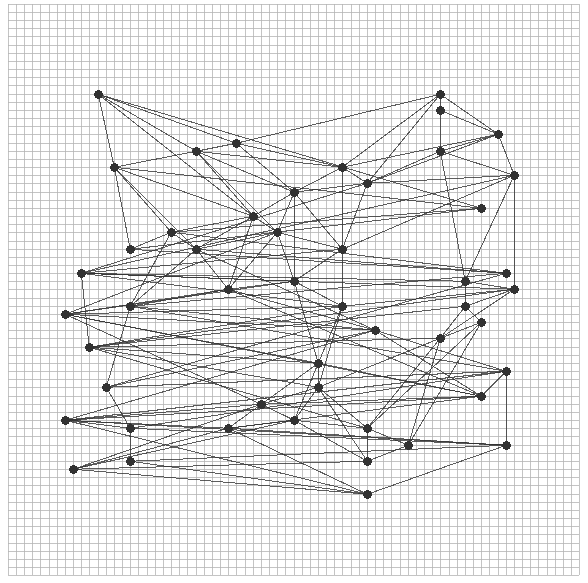
\includegraphics[width=6cm]{g5_initial.PNG}
\caption{Graph 5 initial output}
\end{minipage}
\begin{minipage}[t]{0.48\textwidth}
\centering
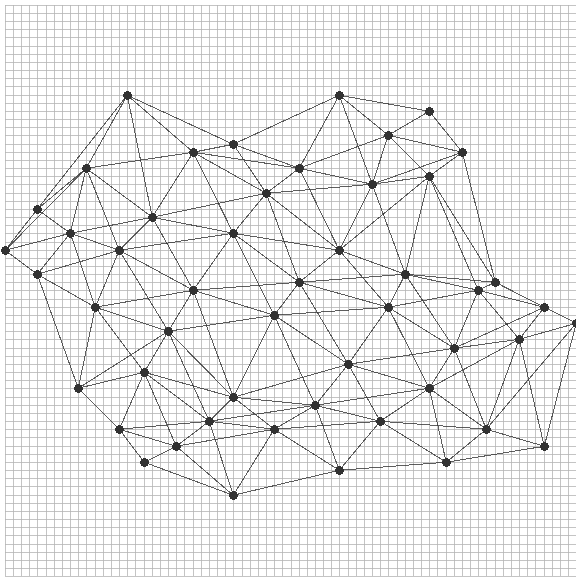
\includegraphics[width=6cm]{g5_FD.png}
\caption{Graph 5 after FD process}
\end{minipage}
\begin{minipage}[t]{0.48\textwidth}
\centering
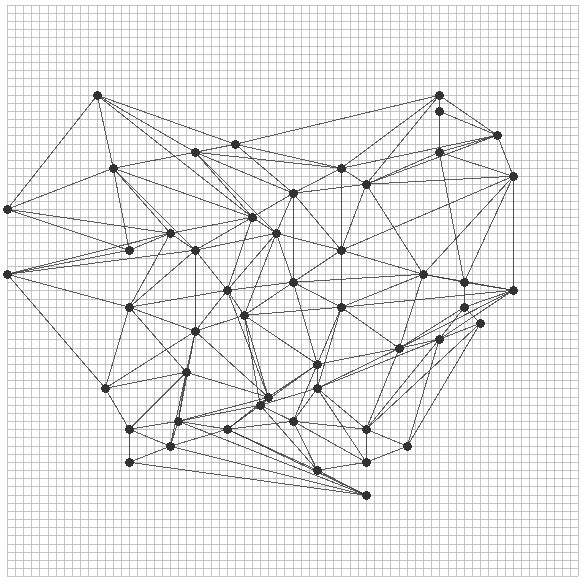
\includegraphics[width=6cm]{g5_LSNode.PNG}
\caption{Graph 5 after LS by nodes process}
\end{minipage}
\begin{minipage}[t]{0.48\textwidth}
\centering
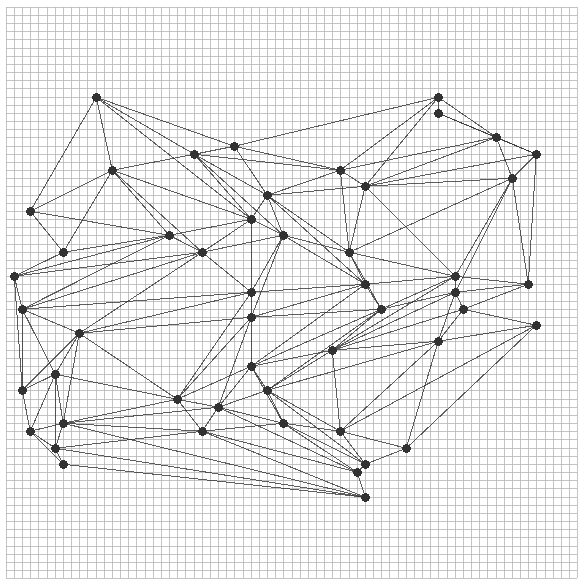
\includegraphics[width=6cm]{g5_LS.PNG}
\caption{Graph 5 after LS by edges process}
\end{minipage}
\end{figure}


\subsection{Time Complexity}

We use a similar table to show the time complexity of these three algorithms in different graph. As our algorithms does not do operations in $y$ axe so we will only look at the graph width. We will also only choose 5 examples with very different dimensions.

\begin{table}[h]
\centering
\begin{tabular}{ p{0.1\textwidth} | p{0.1\textwidth} | p{0.1\textwidth}| p{0.1\textwidth}| p{0.12\textwidth}| p{0.12\textwidth} | p{0.12\textwidth}}
     \hline
     Graph number & Width & Number of nodes & Number of edges & FD result (ms) & LS by nodes result (ms) & LS by edges result (ms)\\
     \hline
     \codeword{2} & 20 & 16 & 42 & 8 & 5 & 366 \\
     \hline
     \codeword{7} & 100000 & 100 & 150 & 120 & 16386 & 7941\\
     \hline
     \codeword{10} & 1000000 & 500 & 684 & 1197  & 190553 & 245671\\
     \hline
     \codeword{11} & 1000000 & 1800 & 6961 & 10724 & 4232 & 2533482\\
     \hline
\end{tabular}
\end{table}

The table tell us:
\begin{enumerate}
    \item The time complexity increase of the FD algorithm is the most stable. Even for large graphs, it can be solved in a reasonable time, but its results may not be very good.
    \item However, the LS by nodes algorithm increase quickly. But if, after a local optimization, the method detects that the results do not improve significantly, the program will end automatically like in Graph 11. It should be noted that although we also set the value of \lstinline{tol} for LS by edge algorithm, but here the \lstinline{tol} is used for step length which will by reduced if the number of intersections augment. Due to the randomness of this algorithm, the chance of not having improvement continuously in several local optimization is very low, so Graph 11 will converge quickly only for LS by nodes algorithm.
    \item The LS by edges algorithm always has a very high time complexity, and this complexity also gives it more outstanding performance.
\end{enumerate}
